
\tikzstyle{simpleNode}=[circle,draw,very thick,minimum width=0.8cm] 

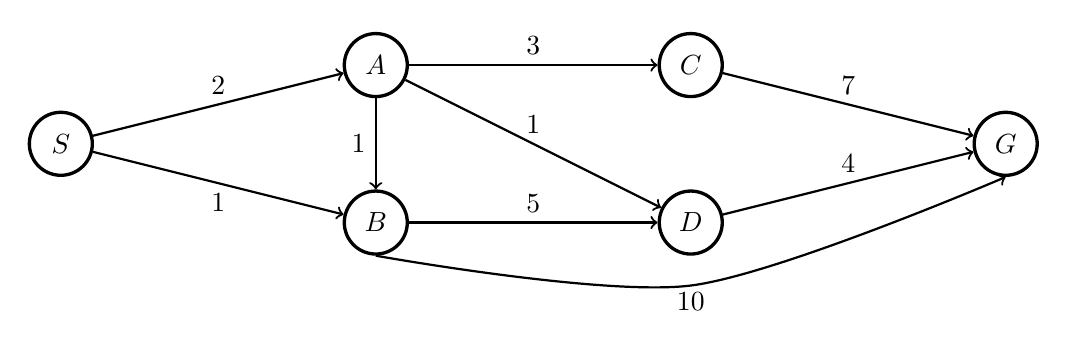
\begin{tikzpicture}[xscale=4,->=stealth]

  \node[simpleNode] (s) at (0,0) {$S$};
  \node[simpleNode] (b) at (1,-1) {$B$};
  \node[simpleNode] (a) at (1,1) {$A$};
  \node[simpleNode] (c) at (2,1) {$C$};
  \node[simpleNode] (g) at (3,0) {$G$};
  \node[simpleNode] (d) at (2,-1) {$D$};
  \path[->,draw,thick] (s)--(a)node[midway,above]{$2$};
  \path[->,draw,thick] (s)--(b)node[midway,below]{$1$};
  \path[->,draw,thick] (a)--(c)node[midway,above]{$3$};
  \path[->,draw,thick] (b)--(d)node[midway,above]{$5$};
  \path[->,draw,thick] (a)--(b)node[midway,left]{$1$};
  \path[->,draw,thick] (a)--(d)node[midway,above]{$1$};
  \path[->,draw,thick] (c)--(g)node[midway,above]{$7$};
  \path[->,draw,thick] (d)--(g)node[midway,above]{$4$};
  \path[->,draw,thick] plot[smooth] coordinates {(b.south) (2,-1.8)(g.south)};
  \node at (2,-2){$10$};
    
\end{tikzpicture}
